\subsection{Faustregel}	\label{subsec:Faustregel}

Als Eselsbrücke zur Bestimmung der Richtung der Feldlinien um den stromdurchflossenen Leiter kann die \glqq Faustregel\grqq{} herangezogen werden. Diese besagt, dass bei der physikalischen Stromrichtung (auch Elektronenflussrichtung genannt) die Feldlinien in Richtung der Fingerspitzen der linken Hand verlaufen, wenn nur der Daumen von der Faust abgespreizt wird und die Flussrichtung angibt.

Für die technische Stromrichtung gilt dieselbe Regel, bloß, dass mit der rechten Faust verfahren wird.

\begin{leftbar}
	Wichtig! Die physikalische Stromrichtung geht von der Bewegung der Elektronen, also der negativen Ladung aus. Diese fließen vom Minuspol zum Pluspol. Die technische Stromrichtung dagegen geht davon aus, dass die positiven Ladungen sich vom Pluspol zum Minuspol bewegen. Durch die Verwendung gespiegelter Handregeln (die jeweils andere Hand wird genommen) bleiben die Effekte jedoch dieselben. 
	
	Allgemein wird in der Physik die physikalische Stromrichtung und damit die \emph{linken} Handregeln bevorzugt, da es auch wirklich die Elektronen sind, die sich in einem Leiter bewegen.
\end{leftbar}


%%!! Cue CUE cue FIX THIS !!%%
\newpage

\subsection{Dauermagneten}  	\label{subsec:DauermagnetFeld}

\endnote{Abbildung \ref{fig:stab} - „VFPt cylindrical magnet thumb“ von Geek3 - Eigenes WerkThis plot was created with VectorFieldPlot. Lizenziert unter CC BY-SA 3.0 über Wikimedia Commons - \url{https://commons.wikimedia.org/wiki/File:VFPt_cylindrical_magnet_thumb.svg}} 
\endnote{Abbildung \ref{fig:hufeisen} - „Feldlinien Hufeisenmagnet“ von unbekannt - unbekannt. Lizenziert unter PD-Schöpfungshöhe über Wikipedia - \url{https://de.wikipedia.org/wiki/Datei:Feldlinien_Hufeisenmagnet.png}}

\begin{figure}[H]
	\centering
	\begin{minipage}[b]{0.45\linewidth}
		\centering
    	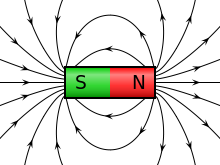
\includegraphics[width=0.9\textwidth]{Stabmagnet}
		\caption{Stabmagnet}
		\label{fig:stab}
	\end{minipage}
	\quad
	\begin{minipage}[b]{0.45\linewidth}
		\centering
    	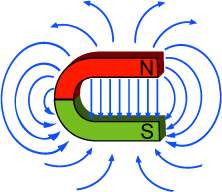
\includegraphics[width=0.8\textwidth]{Hufeisen}
		\caption{Hufeisen: homogener Bereich zwischen den Schenkeln.}
		\label{fig:hufeisen}
	\end{minipage}
\end{figure}


\subsection{Gerader Leiter}
\endnote{„Gerader leiter“ von Talos aus der deutschsprachigen Wikipedia. Lizenziert unter CC BY-SA 3.0 über Wikimedia Commons - \url{https://commons.wikimedia.org/wiki/File:Gerader_leiter.svg}} 
\endnote{„Stromschleife“ von 30px MovGP0 - selbst erstellt mit Inkscape. Lizenziert unter CC BY-SA 2.0 de über Wikimedia Commons - \url{https://commons.wikimedia.org/wiki/File:Stromschleife.svg}} 
\label{subsec:GeraderLeiterFeld}

\begin{figure}[H]
	\centering
	\begin{minipage}[b]{0.45\linewidth}
		\centering
   		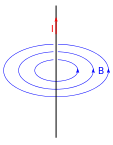
\includegraphics[width=0.7\textwidth]{GeraderLeiter}
		\caption{Geraden Leitern: $I$ zeigt die \emph{technische} Stromrichtung an.}
	\end{minipage}
	\quad
	\begin{minipage}[b]{0.45\linewidth}
		\centering
    	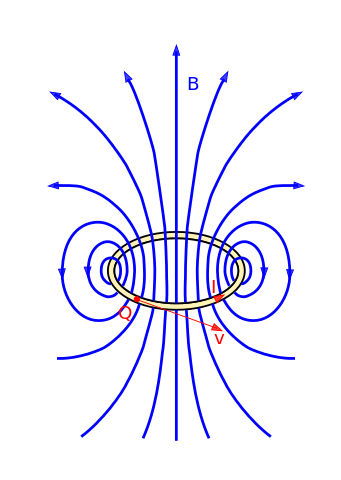
\includegraphics[width=0.7\textwidth]{Stromschleife}
		\caption{Leiterschleife (Spule mit \emph{einer} Windung): Akkumulation zu einem Bündel Feldlinien. Technische Stromrichtung}
	\end{minipage}
\end{figure}

\subsection{Spule} \label{subsec:MFeldSpule}
\endnote{„VFPt cylindrical coil real“ von Geek3 - Eigenes WerkThis plot was created with VectorFieldPlot. Lizenziert unter CC BY-SA 3.0 über Wikimedia Commons - \url{https://commons.wikimedia.org/wiki/File:VFPt_cylindrical_coil_real.svg}}
\label{subsec:Spule}

\begin{figure}[H]
	\centering
   	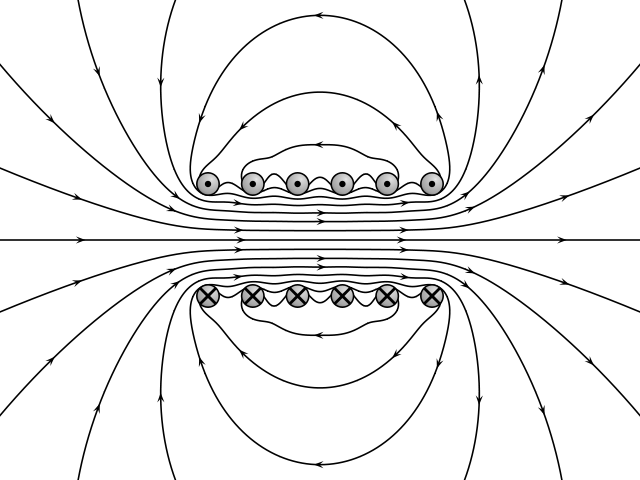
\includegraphics[width=0.55\textwidth]{Spule}
		\caption{Spule: Im Querschnitt zeigt $\otimes$ den technischen Stromfluss \emph{in} die Blattebene an. Vergleich mit Leiterschleife: homogenerer Fluss im Inneren.}
\end{figure}



